\documentclass[11pt,a4paper]{book}
\usepackage{Appunti_universitari}

\begin{document}
\title{Interazione uomo macchina}
\author{Jacopo De Angelis}
\maketitle

\pagebreak
\tableofcontents
\pagebreak

\chapter{Modulo 1: Concetti di base}
\section{Cos'è l'interazione uomo macchina?}
\begin{center}
Definizione standard 

\textit{"HCI (Human-Computer Interaction) è una disciplina che si occupa della progettazione, realizzazione e valutazione di sistemi interattivi con capacità computazionali destinati all'uso umano e dello studio dei principali fenomeni che li circondano"} - \textit{Associacion for Computing Machinery}
\end{center}

L'usabilità di un sistema è spesso trascurata all'interno dell'ambito lavorativo italiano, non per faciloneria ma perchè le risorse da adibire a questo ambito sono una spesa che non viene vista come essenziale nella produzione del valore per andare avanti. 

Il problema viene aggravato dall'outsourcing verso paesi dove il costo del lavoro sia inferiore e, ultimamente, anche da sistemi di ML che sono in grado, con grado di precisione sempre maggiore grazie al deep learning, di sviluppare codice funzionante. Ma cosa viene assegnato ai lavoratori esterni? Ciò che è altamente formalizzato, in modo da lasciare poche possibilità di variazione dalle richieste dei clienti.

Cosa rimane difficile da esternalizzare? Il contatto del cliente, sia durante la prima raccolta di requisiti funzionali, sia le successive interazioni con esso per cambiamenti incrementativi, variazioni di funzionalità o feedback.

L'usabilità è quella caratteristica che rende "facile la vita" al cliente.

\noindent\rule{\textwidth}{1pt}
\begin{center}
\textit{Piccola digressione}
\end{center}
\textbf{Perchè la concorrenza moderna rende sempre più importante l'analisi dell'interazione uomo macchina?}

In un contesto monopolistico le aziende non sono invogliate a produrre la soluzione "migliore"\footnote{Dove per migliore si intende quella che prende in considerazione più metriche come usabilità, efficienza, efficacia, design, ecc} ma solo quella più efficiente a livello di costo marginale.   

Cosa vuole dire questo? Che nella moderna concorrenza derivante da sistemi di sviluppo sempre più semplici e un'offerta più rapida tramite internet, per ottenere quote di mercato le aziende devono iniziare a pensare non solo al "funziona?" ma anche al "come lo faccio funzionare?"
\\\noindent\rule{\textwidth}{1pt}

\textbf{"Qui non si impara a fare delle interfacce usabili, si impara a riconoscere l'usabilità delle interfacce"} ovvero impariamo strumenti che ci possono portare a fare delle belle interfacce, certo, ma soprattutto ci permette di riconoscere cosa renda \underline{buona} un'interfaccia.

La disciplina nasce negli anni '80 ma l'interazione con le macchine (intese come calcolatori) esiste dagli anni'40, semplicemente prima l'utente era ultra specializzato mentre ora quasi tutti possono accedere ad un PC e con questo interagire tramite un'interfaccia.

Dal 1983 si tiene la conferenza annuale \href{https://dl.acm.org/conference/chi}{ACM CHI}. In questi casi tre aree disciplinari si incontrano:
\begin{itemize}
	\item ergonomia
	\item informatica
	\item psicologia comportamentista
\end{itemize}
\begin{figure}[h!]
	\begin{center}
		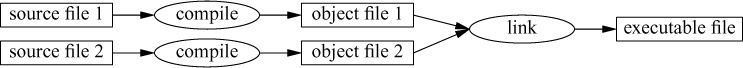
\includegraphics[scale=0.6]{img/001.jpg}
		\caption{HCI e le sue componenti}
		\label{fig: 001}
	\end{center}
\end{figure}
Dobbiamo ricordare sempre una cosa: dobbiamo lasciarci alle spalle l'utente ideale, l'utente senza faccia e senza capacità, e iniziare a pensare all'utente reale, ovvero a chi, idealmente, è diretta la nostra interfaccia. \underline{L'utente non siamo noi}. Proprio per questo le interviste, i test con esterni, i mockup sono utili, perchè ci permettono di vedere la nostra idea attraverso gli occhi di altri. Esempio banale: la nostra interfaccia basata sul colore potrebbe essere altamente confusionaria per un daltonico. Un'applicazione mobile dove tutti i comandi sono sulla destra potrebbe essere difficile da usare per un mancino.

\textbf{Ergonomia cognitiva}: studio dell'interazione tra l'uomo e gli strumenti per l'elaborazione di informazioni studiando i processi cognitivi coinvolti (percezione, attenzione, memoria, pensiero, linguaggio, emozioni) e suggerendo delle soluzioni per migliorare tali strumenti.

\section{Perchè è difficile progettare perchè l'interazione sia "buona"?}
Ci sono tre ragioni, idealmente:
\begin{enumerate}
	\item \textbf{La varietà dei sistemi interattivi}: cellulari, computer, cloche, macchine da cucina, tablet...
	\item \textbf{La varietà degli utenti}: fasce d'età, background culturale, condizioni mediche...
	\item \textbf{La varietà degli scopi e degli usi}: contesti formativi, ludici, lavorativi e usi tramite dispositivi diversi, in luoghi differenti...
\end{enumerate}

\begin{center}
\textbf{\textit{Noi studieremo come progettare per la varietà e al volto delle procedure.}}
\end{center}

\section{Temi dell'HCI}
\begin{itemize}
	\item Criteri, metodi e strumenti per la \underline{progettazione dell'interazione} fra esseri umani e sistemi interattivi. L'interazione è il contesto nel quale interagiamo;
	\item Criteri, metodi e strumenti per la \underline{valutazione dell'usabilità} dei sistemi interattivi;
	\item Progettazione di nuove \underline{tecniche di interazione} (dall'hololens ai sistemi che sfruttano i sistemi nervosi);
	\item Valutazione dell'\underline{impatto dell'automazione} nei contesti umani
	\item \underline{Sistema socio-tecnico}
\end{itemize}
Per valutazione dell'\textbf{impatto} ci si riferisce a due tipi di impatto:
\begin{itemize}
	\item a breve termine: sui singoli e nel qui ed ora (usabilità)
	\item a medio-lungo termine: sono conseguenze inattese sulla collettività
\end{itemize}

\noindent\rule{\textwidth}{1pt}
\begin{center}
	\textbf{Errore comune}
\end{center}

L'usabilità è un tipo di effetto/impatto sugli utenti (sui singoli utenti), NON è una caratteristica intrinseca di un sistema). Per questo non si può valutare l'usabilità senza il coinvolgimento degli utenti (di vario tipo) e sarebbe meglio valutarla in un contesto più simile possibile a una situazione reale.

Ricordiamo che l'usabilità non è solo un concetto di "correttezza funzionale" ma anche di "facilità d'uso".

\noindent\rule{\textwidth}{1pt}

Non si può parlare di impatto se non si parla di su che sistema socio-tecnico dovrà avere un impatto.
\subsection{Sistema socio-tecnico}
Banalmente possiamo dire che è un contesto di umani che lavorano assieme tramite delle tecnologie. Quindi:
\begin{itemize}
	\item è un sistema, "un insieme di elementi interrelati ed eventualmente mutuamente dipendenti che, agli occhi di un osservatore esterno, appaiono come un'entità unitaria ma collettiva, con caratteristiche e comportamento proprio, solitamente autonomo ed intenzionale (cioè volto ad un obiettivo)";
	\item Un sistema in cui la componente umana  (sociale) e quella tecnica (tecnologica) sono inestricabilmente legate tra loro e la loro interazione porta a fenomeni emergenti impredicibili. Attenzione che tecnica è un termine generico proprio per intendere tutti gli strumenti, che siano fisici o dell'ingegno. In più si parla di interdipendenza perchè lo strumento è fermo senza qualcuno che lo usa, l'umano è fermo se non ha uno strumento per agire;
	\item è un concetto di invarianza di scala, ovvero il concetto non cambia in base alla grandezza dell'ambiente sociale
\end{itemize}
Come progettisti dobbiamo essere pronti all'imprevisto, ovvero all'utente che usa lo strumento non nel modo prescritto.

STS\footnote{Socio-technical system} thinking: un approccio che è consapevole che le due componenti si integrano bene (fit) e si "ottimizzano" solo congiuntamente in configurazioni subottime (joint optimization). Bisogna quindi pensare al sistema nella sua interezza e come le parti si integreranno.

Non si deve pensare solo alla qualità degli strumenti ma anche al contesto nel quale vanno usati. Ad esempio la soddisfazione del lavoratore può migliorare l'interazione. Questo va a contribuire alla qualità della configurazione. 

L'introduzione di una tecnologia in un contesto (sociale) è parte di un processo di cambiamento operante su più piani. Seguendo ciò che è detto prima si capisce che bisogna pensare non solo alla nostra tecnologia a livello funzionale (sistema tecnico) quando pensiamo all'interazione ma anche a dove andrà inserita e come migliorare quel contesto (sistema sociale).
 
\subsection{Proprietà emergenti}
Sono di due tipi:
\begin{itemize}
	\item \textbf{Sono proprietà funzionali}, riguardano il funzionamento dell'intero sistema una volta che tutte le sue parti, assembrale come devono, funzionano bene.
	\item \textbf{Sono proprietà non funzionali} che riguardano quanto bene opera il sistema in un determinato ambiente/contesto. Un elenco non esaustivo è affidabilità, sicurezza, performance, sicurezza, usabilità, comfort. (E.g. le informazioni sono giuste ma non aggiornate in un sistema medico, perchè? Perchè non era comodo farlo, quindi veniva visto più come un obolo rispetto ad uno strumento utile, vuole dire che è progettato male a livello di usabilità)
\end{itemize}

\begin{center}
	\textit{L'emergenza è quando la somma delle parti vale più (a livello di usabilità) delle parti singole (e.g. una bici e le sue parti)}
\end{center}



\end{document}